\section{Experimental Demonstration}\label{sec: experiments}
The environment that the learning agent is facing in our experiments
is based on a type of transportation domain that in its general form
can represent a wide range of practical tasks from a real
transportation route planning to the manipulator motion planning for a
robot. To better demonstrate the properties and the performance of our
teaching method, rather than to deal with various intricacies of the
domain, we concentrate on a discrete version of the
task. Specifically, consider a learner agent that is tasked with
finding an optimal path for supply transportation between point $S$
and $T$ on a grid. The learner's reward is initially fixed to be $-1$
for every step it takes plus some values $R_{ST}$ and $R_{TS}$ for
reaching point T from S and vice versa. In a uniform grid this would
be a simple problem, however, the grid simulates a terrain and cells
have an associated elevation.  As a result, any movement from one cell
to another neighbouring cell succeeds with a probability proportional
to the relative elevation of the cells. This way we can, for example,
simulate and model the resistance presented by a real rugged or
mountain terrain to the efforts of a robot that attempts to traverse
it. From this point of view, consider, for instance, the situation
depicted in Figure~\ref{exp_motion}.

\begin{figure}[ht]
\centerline{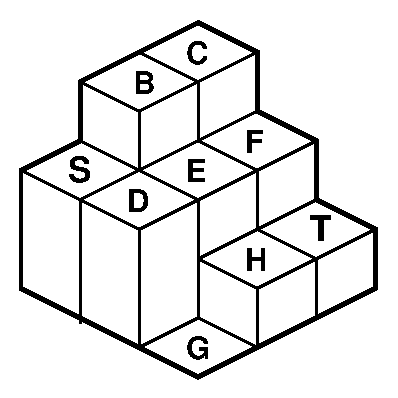
\psfig{file=img/exp_motion.eps,width=5cm}}
\caption{\label{exp_motion}Example of a 3D terrain grid.}
\end{figure}

If the cells are of equal elevation, the movement almost always
succeeds, in particular moving from cell $B$ to cell $C$ in
Figure~\ref{exp_motion} is practically certain. If the source cell of
the motion is lower than the target cell, then the motion succeeds
with low probability. Furthermore, in this case, a non-zero
probability exists that the direction of motion will be
altered. E.g. moving from $H$ to $E$ is unlikely to succeed, and the
agent may end up in $D$, $F$ or even $G$, thus representing a robot
``stumbling'' or ``slipping'' while trying to climb a steeply inclined
slope. If the motion is directed to lower the elevation, it is most
likely will succeed, but it also has a certain non-negligible
probability to move further than intended. E.g. moving from $B$ to $E$
is quite likely to succeed, but the agent may end up in $H$ or $G$
just as well, which would also be consistent with a real motion on a
steep mountain slope.

As a result of this non-uniform, and potentially even non-linear,
response to actions, such an environment can create complex
dependencies between motion decision at different locations on the
grid. Finding an optimal path of motion from $S$ to $T$ and back,
therefore, becomes non-trivial. Still, if the probabilities of
different transitions are given, the policy iteration algorithm can
comfortably well solve the problem. However, the time it takes the
algorithm to converge to an optimal policy may vary depending on how
prominent are the features of the terrain. Therefore it would be
reasonable to assume that scaling the terrain (and modifying
transition probabilities accordingly) during the initial iterations of
learning, or shaping the landscape to ``push'' the agent in the right
direction will result in faster convergence to the optimal
solution. Our experiments are directed to verify this proposition
using our TOP-PI formalism.  Furthermore, to demonstrate that the
teacher can indeed cultivate a given behaviour to the degree of actually 
enforcing it, we consider the situation where the learner is required
to follow a path different to what would be optimal with respect to
the environment's passive dynamics. %We also test the efficacy of
%directing the agent to follow a specific path, different to the
%optimal, from $S$ to $T$ using TOP-PI.

We begin our experimental verification by considering a $4 \times 4$
grid world where the learner can move in any cardinal direction or
stay put.  Each cell has a randomly assigned elevation, shown in
Figure~\ref{probalt}, that modifies the dynamics of each action as
described above.  The learner has a reward of $+1$ for any actions
ending in the target state and $-1$ otherwise.  This results in an
optimal policy of heading toward the target state in the shortest
number of steps (see Figure~\ref{prevopt}).  The learner uses policy
iteration to find a behaviour policy that maximises the expected
discounted sum of future rewards. The teacher can arbitrarily modify
the underlying dynamics of the environment.

\begin{figure}[ht]
\centerline{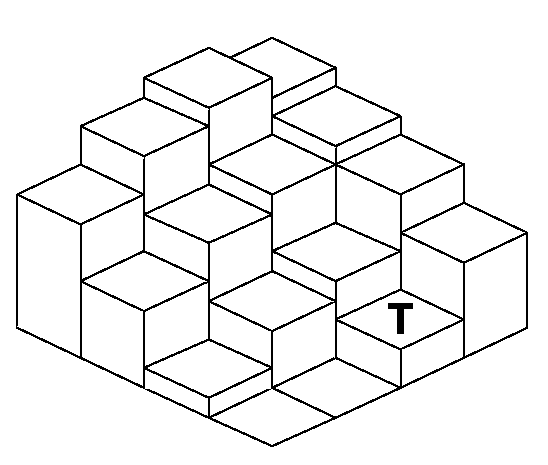
\psfig{file=img/probalt.eps,width=5cm}}
\caption{\label{probalt}The unmodified 3D terrain.}
\end{figure}

\begin{figure}[ht]
\centerline{
\psfig{file=img/prevopt.eps,width=5cm}}
\caption{\label{prevopt}Original optimal policy of our test grid.  The shaded cell is the target state, with the policy action to remain put.}
\end{figure}

In our test environment, the information about the reward state can
take multiple iterations of the PI algorithm to propagate to all other
states.  This leaves the learner to make arbitrary guesses in early
iterations.  By using TOP-PI, we found that the teacher was able to
shape the dynamics such that the agent is ``pushed'' in the
appropriate direction from the beginning.  Without the teacher
modifying the dynamics, the learner required $4$ iterations of PI to
find the optimal policy.  With the addition of the teacher, the
modified dynamics led the learner to follow the target policy in $3$
iterations.

\begin{figure}[ht]
\centerline{
\psfig{file=img/newopt.eps,width=5cm}}
\caption{\label{newopt}A target policy that avoids centre cells.}
\end{figure}

\begin{figure}[ht]
\centerline{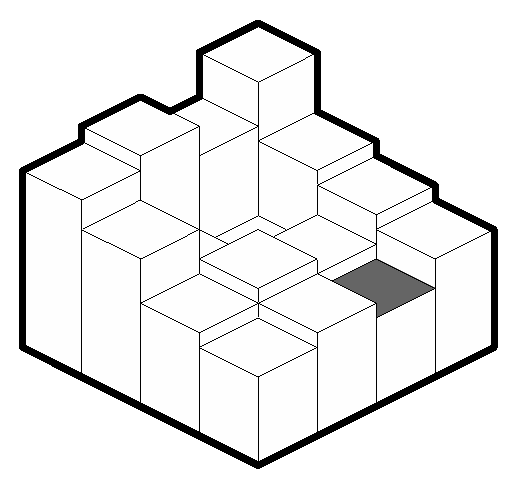
\psfig{file=img/newalt.eps,width=5cm}}
\caption{\label{newalt}An impression of the new terrain corresponding to the modified dynamics at the final iteration.}
\end{figure}

However, the significance of the teacher's tweaks can be better
appreciated if we consider the fact that it can, instead of
facilitating, distort the learning process. Therefore, we tested our
TOP-PI solution in the situation where the required policy was
different from the optimal trajectory in the environment with passive
dynamics. Specifically, we tasked our algorithm to divert the PI
learner from a simple shortest path to the reward state to one that
avoids the centre states and follows the edge states to the goal (see
Figure~\ref{newopt}).  Our tests showed that this policy modification
was indeed achievable through the modifications, provided by the
teacher, to the environment dynamics.  With the teacher using TOP-PI
on the new target policy, the learner found this new policy using
Policy Iteration in $4$ iterations. This is the same time it took to
find the shortest path policy, in spite of the new target policy being
a distorted one.  Although in these experiments the tweaked dynamics
were not computed based on some underlying terrain, the tweaked
dynamics of the final policy iteration are visualised by a terrain
impression shown in Figure~\ref{newalt}.  Note the lowering of the two
centre states furthest from the target.  This creates a ``hole'' that
the learner would wish to avoid as it would be difficult to exit.
Also, the upper-right centre square is the lowest to discourage the
learner from moving there should it fall in the hole. In this domain
with a maximum number of policy iterations for TOP-PI of $4$ the
modifications to the dynamics tended to be relatively reasonable, with
the average change in each entry of the environmental dynamics $T$
ranging from $0.058$ in the first iteration to $0.036$ in the final
iteration. However, the effort invested by the teacher can be better
appreciated with that of facilitating the shortest path
problem. While in our first experiment the cumulative KLR-based cost
to the teacher was $2.1495$ units, the distorted policy required
$7.1685$ units of teaching effort.

However, we reduced the grid size to $2\times 2$ to underline and throw
into a sharper relief the fact that this policy modification method
allows changes that are not possible with modifications to the reward
function alone. In our test on a $2 \times 2$ grid, we changed the
policy from a shortest path to a circular motion (see
Figure~\ref{envdopt}), almost reversing the learner's motion
tendencies under the passive environment dynamics. On the other hand,
consider the current state of the art in the {\em incentive} based
environment design, where reward augmentation is parameterised by
state. To achieve the required circular policy by modifying the reward
function, the reward values must be strictly increasing along the
path, otherwise it would be optimal to remain put. By following the
circular motion, it is necessary for the reward in the upper-left
state to be less than the reward for the lower right (target)
state. As a result the optimal action for lower-left state would
inevitably be to move right rather than up, thus failing to induce the
required circular motion. However, as we have demonstrated, tweaking
the dynamics allows such a policy modification.

\begin{figure}[ht]
\centerline{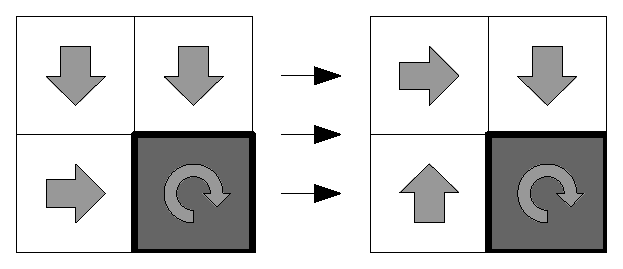
\psfig{file=img/envdopt.eps,width=5cm}}
\caption{\label{envdopt}The original optimal policy (left) and target policy (right).}
\end{figure}

Our experiments provided experimental verification of our proposed
{\em behaviour cultivation} teaching method.  We verified that the
method can be used both to speed up the learning process and to lead
it towards a required strategy by applying our method to the Policy
Iteration algorithm. We have confirmed the efficacy of our method in
the situation where the teacher's interest contradicts, or otherwise
interferes, with the interests of the learner by requiring to
cultivate a behaviour significantly different from that which is
optimal under the passive environment dynamics. Importantly, we have
constructed a teacher-learner task that can not be addressed by other
available teaching methods.
